
% \titlegraphic{\hfill\includegraphics[height=1.5cm]{logo.pdf}}

\documentclass[xcolor=pdftex,dvipsnames,table,numbers,hyperref={pdfpagelabels=false},compress]{beamer}
%\usepackage{requiredPackage}
\usepackage{amsmath}
\usepackage{graphicx}
\usepackage{amsfonts}
\usepackage{amssymb}

\usepackage{tabularx}
\usepackage{epstopdf}
\usepackage{overpic}
\usepackage{url}
\usepackage{calrsfs}
\usepackage{mathrsfs}
\usepackage{epsfig}
\usepackage{cancel}
\usepackage{changepage}

\usepackage{tikz}
\usepackage[customcolors]{hf-tikz} 

\usepackage{lmodern}
%\usepackage{mystyle}
\usepackage{subfig}
\usepackage{pifont}
\usepackage{tabu}
\usepackage{xcolor}
\usepackage{algorithm}
\usepackage{algpseudocode}
%\usepackage{enumitem}
\usepackage{remreset}
\usepackage{etoolbox}
\usepackage{comment} % end and begin comment
%\usepackage{dtklogos} 
\usepackage{listings}
\lstset{breaklines=true} 

\newcommand{\gline}{\textcolor{gray}{\hline}}
\newcommand{\cmark}{\ding{51}}%
\newcommand{\xmark}{\ding{55}}%
\newcommand{\gcheck}{\textcolor{blue}{\Large \cmark}}
\newcommand{\rcross}{\textcolor{red}{\Large \xmark}}
\newcommand{\tkt}{\tilde{K}_\theta}
\newcommand{\kt}{K_\theta}
\newcommand{\ind}{\overset{ind}{\sim}}
\newcommand{\plim}{\overset{p}{\rightarrow}}
\newcommand{\cx}{\frac {X'X}n}
\newcommand{\cz}{\frac {Z'Z}n}
\newcommand{\ccz}{\frac {Z'Z}n - \Sigma_A}
\newcommand{\czy}{\frac {Z'y}n}
\newcommand{\cyz}{\frac {y'Z}n}
\newcommand{\cxy}{\frac {X'y}n}
\newcommand{\cyx}{\frac {y'X}n}
\newcommand{\myitem}{\vskip3mm \item}

\newcommand{\calS}{{\cal S}}
\newcommand{\calA}{{\cal A}}
\newcommand{\calK}{{\cal K}}
\newcommand{\calX}{{\cal X}}
\newcommand{\calD}{{\cal D}}
\newcommand{\calG}{{\cal G}}
\newcommand{\calT}{{\cal T}}
\newcommand{\calU}{{\cal U}}
\newcommand{\calR}{{\cal R}}
\newcommand{\tp}{\tilde{p}}
\newcommand{\tildebC}{\tilde{\bC}}
\newcommand{\calL}{{\cal L}}

\newcommand{\blam}{ \mbox{\boldmath $ \lambda $} }
\newcommand{\bet}{ \mbox{\boldmath $ \eta $} }
\newcommand{\bome}{ \mbox{\boldmath $ \omega $} }
\newcommand{\bbet}{ \mbox{\boldmath $ \beta $} }
\newcommand{\bbeta}{ \mbox{\boldmath $ \beta $} }
\newcommand{\balph}{ \mbox{\boldmath $ \alpha $} }
\newcommand{\balpha}{ \mbox{\boldmath $ \alpha $} }
\newcommand{\bphi}{ \mbox{\boldmath $\phi$}}
\newcommand{\bzeta}{ \mbox{\boldmath $\zeta$}}
\newcommand{\bkap}{ \mbox{\boldmath $\kappa$}}
\newcommand{\bkappa}{ \mbox{\boldmath $\kappa$}}
\newcommand{\beps}{ \mbox{\boldmath $\epsilon$}}
\newcommand{\bepsilon}{ \mbox{\boldmath $\epsilon$}}
\newcommand{\bthet}{ \mbox{\boldmath $ \theta $} }
\newcommand{\btheta}{ \mbox{\boldmath $ \theta $} }
\newcommand{\blambda}{ \mbox{\boldmath $ \lambda $} }
\newcommand{\bnu}{ \mbox{\boldmath $\nu$} }
\newcommand{\bmu}{ \mbox{\boldmath $\mu$} }
\newcommand{\bGam}{ \mbox{\boldmath $\Gamma$} }
\newcommand{\bSig}{ \mbox{\boldmath $\Sigma$} }
\newcommand{\bSigma}{ \mbox{\boldmath $\Sigma$} }
\newcommand{\bPhi}{ \mbox{\boldmath $\Phi$} }
\newcommand{\bThet}{ \mbox{\boldmath $\Theta$} }
\newcommand{\bTheta}{ \mbox{\boldmath $\Theta$} }
\newcommand{\bDel}{ \mbox{\boldmath $\Delta$} }
\newcommand{\bDelta}{ \mbox{\boldmath $\Delta$} }
\newcommand{\bnabla}{ \mbox{\boldmath $\nabla$} }
\newcommand{\bLam}{ \mbox{\boldmath $\Lambda$} }
\newcommand{\bLambda}{ \mbox{\boldmath $\Lambda$} }
\newcommand{\bgam}{ \mbox{\boldmath $\gamma$} }
\newcommand{\bgamma}{ \mbox{\boldmath $\gamma$} }
\newcommand{\brho}{ \mbox{\boldmath $\rho$} }
\newcommand{\bdel}{ \mbox{\boldmath $\delta$} }
\newcommand{\bdelta}{ \mbox{\boldmath $\delta$} }
\newcommand{\sis}{\sigma^2}
\newcommand{\bOmega}{\mbox{\boldmath $\Omega$} }
\newcommand{\bPsi}{ {\boldsymbol \Psi} }
\newcommand{\btkt}{\boldsymbol{\tilde{K}}_\theta}
\newcommand{\pg}{P{\'o}lya-Gamma }

\newcommand{\bzero}{\textbf{0}}
\newcommand{\bones}{\textbf{1}}
\newcommand{\ba}{\textbf{a}}
\newcommand{\bb}{\textbf{b}}
\newcommand{\bB}{\textbf{B}}
%\newcommand{\bA}{\textbf{A}}
\newcommand{\bc}{\textbf{c}}
\newcommand{\bC}{\textbf{C}}
\newcommand{\bA}{\textbf{A}}
\newcommand{\bd}{\textbf{d}}
\newcommand{\bD}{\textbf{D}}
\newcommand{\be}{\textbf{e}}
\newcommand{\bE}{\textbf{E}}
\newcommand{\bk}{\textbf{k}}
\newcommand{\bK}{\textbf{K}}
\newcommand{\bh}{\textbf{h}}
\newcommand{\bs}{\textbf{s}}
\newcommand{\bS}{\textbf{S}}
\newcommand{\bH}{\textbf{H}}
\newcommand{\bI}{\textbf{I}}
\newcommand{\bt}{\textbf{t}}
\newcommand{\bu}{\textbf{u}}
\newcommand{\bv}{\textbf{v}}
\newcommand{\bw}{\textbf{w}}
\newcommand{\bW}{\textbf{W}}
\newcommand{\bx}{\textbf{x}}
\newcommand{\bX}{\textbf{X}}
\newcommand{\by}{\textbf{y}}
\newcommand{\bY}{\textbf{Y}}
\newcommand{\bz}{\textbf{z}}
\newcommand{\bZ}{\textbf{Z}}
\newcommand{\bL}{\textbf{L}}
\newcommand{\br}{\textbf{r}}
\newcommand{\bR}{\textbf{R}}
\newcommand{\bm}{\textbf{m}}
\newcommand{\bM}{\textbf{M}}
\newcommand{\given}{\,|\,}
\newcommand{\T}{\top}
\newcommand{\bV}{\textbf{V}}
\newcommand{\bJ}{\textbf{J}}
\newcommand{\blue}[1]{{\color{RoyalBlue!90} #1}}
\newcommand{\red}[1]{{\color{Red} #1}}
\newcommand{\green}[1]{{\color{Green} #1}}
\newcommand{\orange}[1]{{\color{Orange} #1}}
\newcommand{\titl}[1]{{\begin{large}\begin{center}#1\end{center}\end{large}}}

\newcommand{\tildea}{\tilde{a}}
\newcommand{\tildeba}{\tilde{\ba}}
\newcommand{\tildebv}{\tilde{\bv}}
\newcommand{\tildev}{\tilde{v}}
\newcommand{\tildeA}{\tilde{A}}
\newcommand{\tildeC}{\tilde{C}}
\newcommand{\tildeK}{\tilde{K}}
\newcommand{\tildew}{\tilde{w}}
\newcommand{\tildeu}{\tilde{u}}
\newcommand{\tildebw}{\tilde{\bw}}
\newcommand{\tildeeps}{\tilde{\epsilon}}
\newcommand{\tildebeps}{\tilde{\bepsilon}}
\newcommand{\eps}{\epsilon}
\newcommand{\sigs}{\sigma^2}
\newcommand{\taus}{\tau^2}
\newcommand{\iid}{\stackrel{\mathrm{iid}}{\sim}}

%\newcommand{\calS}{{\cal S}}
\newcommand{\calC}{{\cal C}}

%\documentclass[10pt]{beamer}

\usetheme{metropolis}
\usepackage{appendixnumberbeamer}

\usepackage{booktabs}
\usepackage[scale=2]{ccicons}

\usepackage{pgfplots}
\usepgfplotslibrary{dateplot}

\usepackage{xspace}
\newcommand{\themename}{\textbf{\textsc{metropolis}}\xspace}

\makeatletter
\@addtoreset{subfigure}{framenumber}% subfigure counter resets every frame
\makeatother

\makeatletter
\@addtoreset{figure}{framenumber}% subfigure counter resets every frame
\makeatother

\setbeamertemplate{caption}{\raggedright\insertcaption\par}
\captionsetup[subfigure]{labelformat=empty}


\title[]{Spatial Factor Models for Multivariate Spatial Data}
\author{Jeffrey Doser$^1$ \& Andrew Finley$^2$}
	
\institute{
\begin{tiny}$^1$Department of Integrative Biology, Michigan State University.\\
$^2$Department of Forestry, Michigan State University.\end{tiny}
}

\date{May 15, 2023}


\begin{document}

\maketitle

\begin{frame}{Multivariate spatial data}

\begin{itemize}
\item Point-referenced spatial data often come as multivariate measurements at each location.\pause

\item Examples:
\begin{itemize}
	\item \red{Environmental monitoring}: stations yield measurements on ozone, NO, CO, and $\text{PM}_{2.5}$.\pause
	\item \red{Community Ecology}: assemblages/communities of species \pause
	\item \red{Forestry}: measurements of stand characteristics age, total biomass, and average tree diameter.\pause
	\item \red{Atmospheric modeling}: at a given site we observe surface temperature, precipitation and wind speed \pause
\end{itemize}

\item We anticipate dependence between measurements %\pause
\begin{itemize}
\item at a particular location%\pause
\item across locations
\end{itemize}
\end{itemize}
\end{frame}

\begin{frame}{Multivariate spatial generalized linear model}

\begin{itemize}
    \item Spatial generalized linear model for $h$-variate spatial data for $j = 1, 2, \dots, h$ and $i = 1, \dots, n$: 
    \begin{align*}
	    y_j(\bs_i) &\sim f(\mu_j(\bs_i), \tau_j) \\
	    \mu_j(\bs_i) &= g^{-1}(\eta_j(\bs_i)) = \bx(\bs_i)^\top\bbeta_j + \text{w}^\ast_j(\bs_i)
    \end{align*}
    \item We can imagine modeling $\bw^\ast(\bs_i) = (\text{w}^\ast_1(\bs_i), \text{w}^\ast_2(\bs_i), \ldots, \text{w}^\ast_h(\bs_i))'$ as an $h$-variate Gaussian process \pause
    \item Could model using Multivariate NNGP as disussed previously with SVCs, works well when $h < 5$. \pause
    \item But what about when $h$ is large (e.g,. 10, 100)?
\end{itemize}
\end{frame}

\begin{frame}{Spatial Factor Model}
    \begin{itemize}
    \item Approximates the dependence between multivariate (spatially-dependent) outcomes through a linear combination of a (much) lower-dimensional set of spatial factors \pause
    \item We represent the $h \times 1$ vector $\bw^\ast(\bs_i)$ as a linear combination of latent spatial factors and factor loadings: 
	    \begin{align*}
                 \bw^\ast(\bs) = \bLambda\bw(\bs_i)
	    \end{align*}
    \item $\bLambda$ is an $h \times q$ loadings matrix (tall and skinny) and $\bw(\bs_j)$ is a $q \times 1$ vector of realizations from $q$ independent spatial GPs \pause
    \item In traditional factor analysis, $\bw(\bs_i)$ are realizations from independent standard normal random variables.
    \end{itemize}
\end{frame}

\begin{frame}{Spatial Factor Model}
   \begin{itemize}
        \item Choosing $q << m$ leads to substantial computational reductions.
	\item Simple to code: just sample from $q$ independent GPs as with basic univariate models.
	\item Yields a non-separable multivariate cross-covariance function given by $\sum_{k = 1}^q\bR_k(\phi_k)\blambda_k\blambda_k^\top$
	\item Can simply replace the $q$ full GPs with their corresponding NNGPs to yield a spatial factor NNGP model
	\item Identifiability constraints on $\bLambda$: fix upper triangle to 0 and diagonal to 1. See Ren and Banerjee (2013) \textit{Biometrics}
   \end{itemize}
\end{frame}

\begin{frame}{Priors}
    \begin{itemize}
	    \item Standard normal priors for the lower triangle of $\bLambda$
	    \item We like to model response-specific regression coefficients $\bbeta_j$ hierarchically. For each $r = 1, \dots, p$ covariate, we model $\beta_{j, r}$ following
		    \begin{align*}
			    \beta_{j, r} \sim N(\mu_{\beta_r}, \tau^2_{\beta_r})
		    \end{align*}
	    \item Gaussian hyperpriors for $\mu_{\beta_r}$ and IG or half-Cauchy priors for $\tau^2_{\beta_r}$
	    \item Independent uniform priors for spatial decay parameters $\bphi$
    \end{itemize}
\end{frame}

\begin{frame}{Why we like spatial factor models}
    \begin{itemize}
         \item Simple to code (don't need to deal with cross-covariance matrices). \pause
	 \item Relatively fast and efficient (well, at least for Gaussian and Binomial). \pause
	 \item Factors and factor loadings can be used for model-based ordination. \pause
	 \item Straightforward extensions to spatially-varying coefficient models.
    \end{itemize}
\end{frame}

\begin{frame}{Example: bird communities across the continental US}
	\begin{center}
             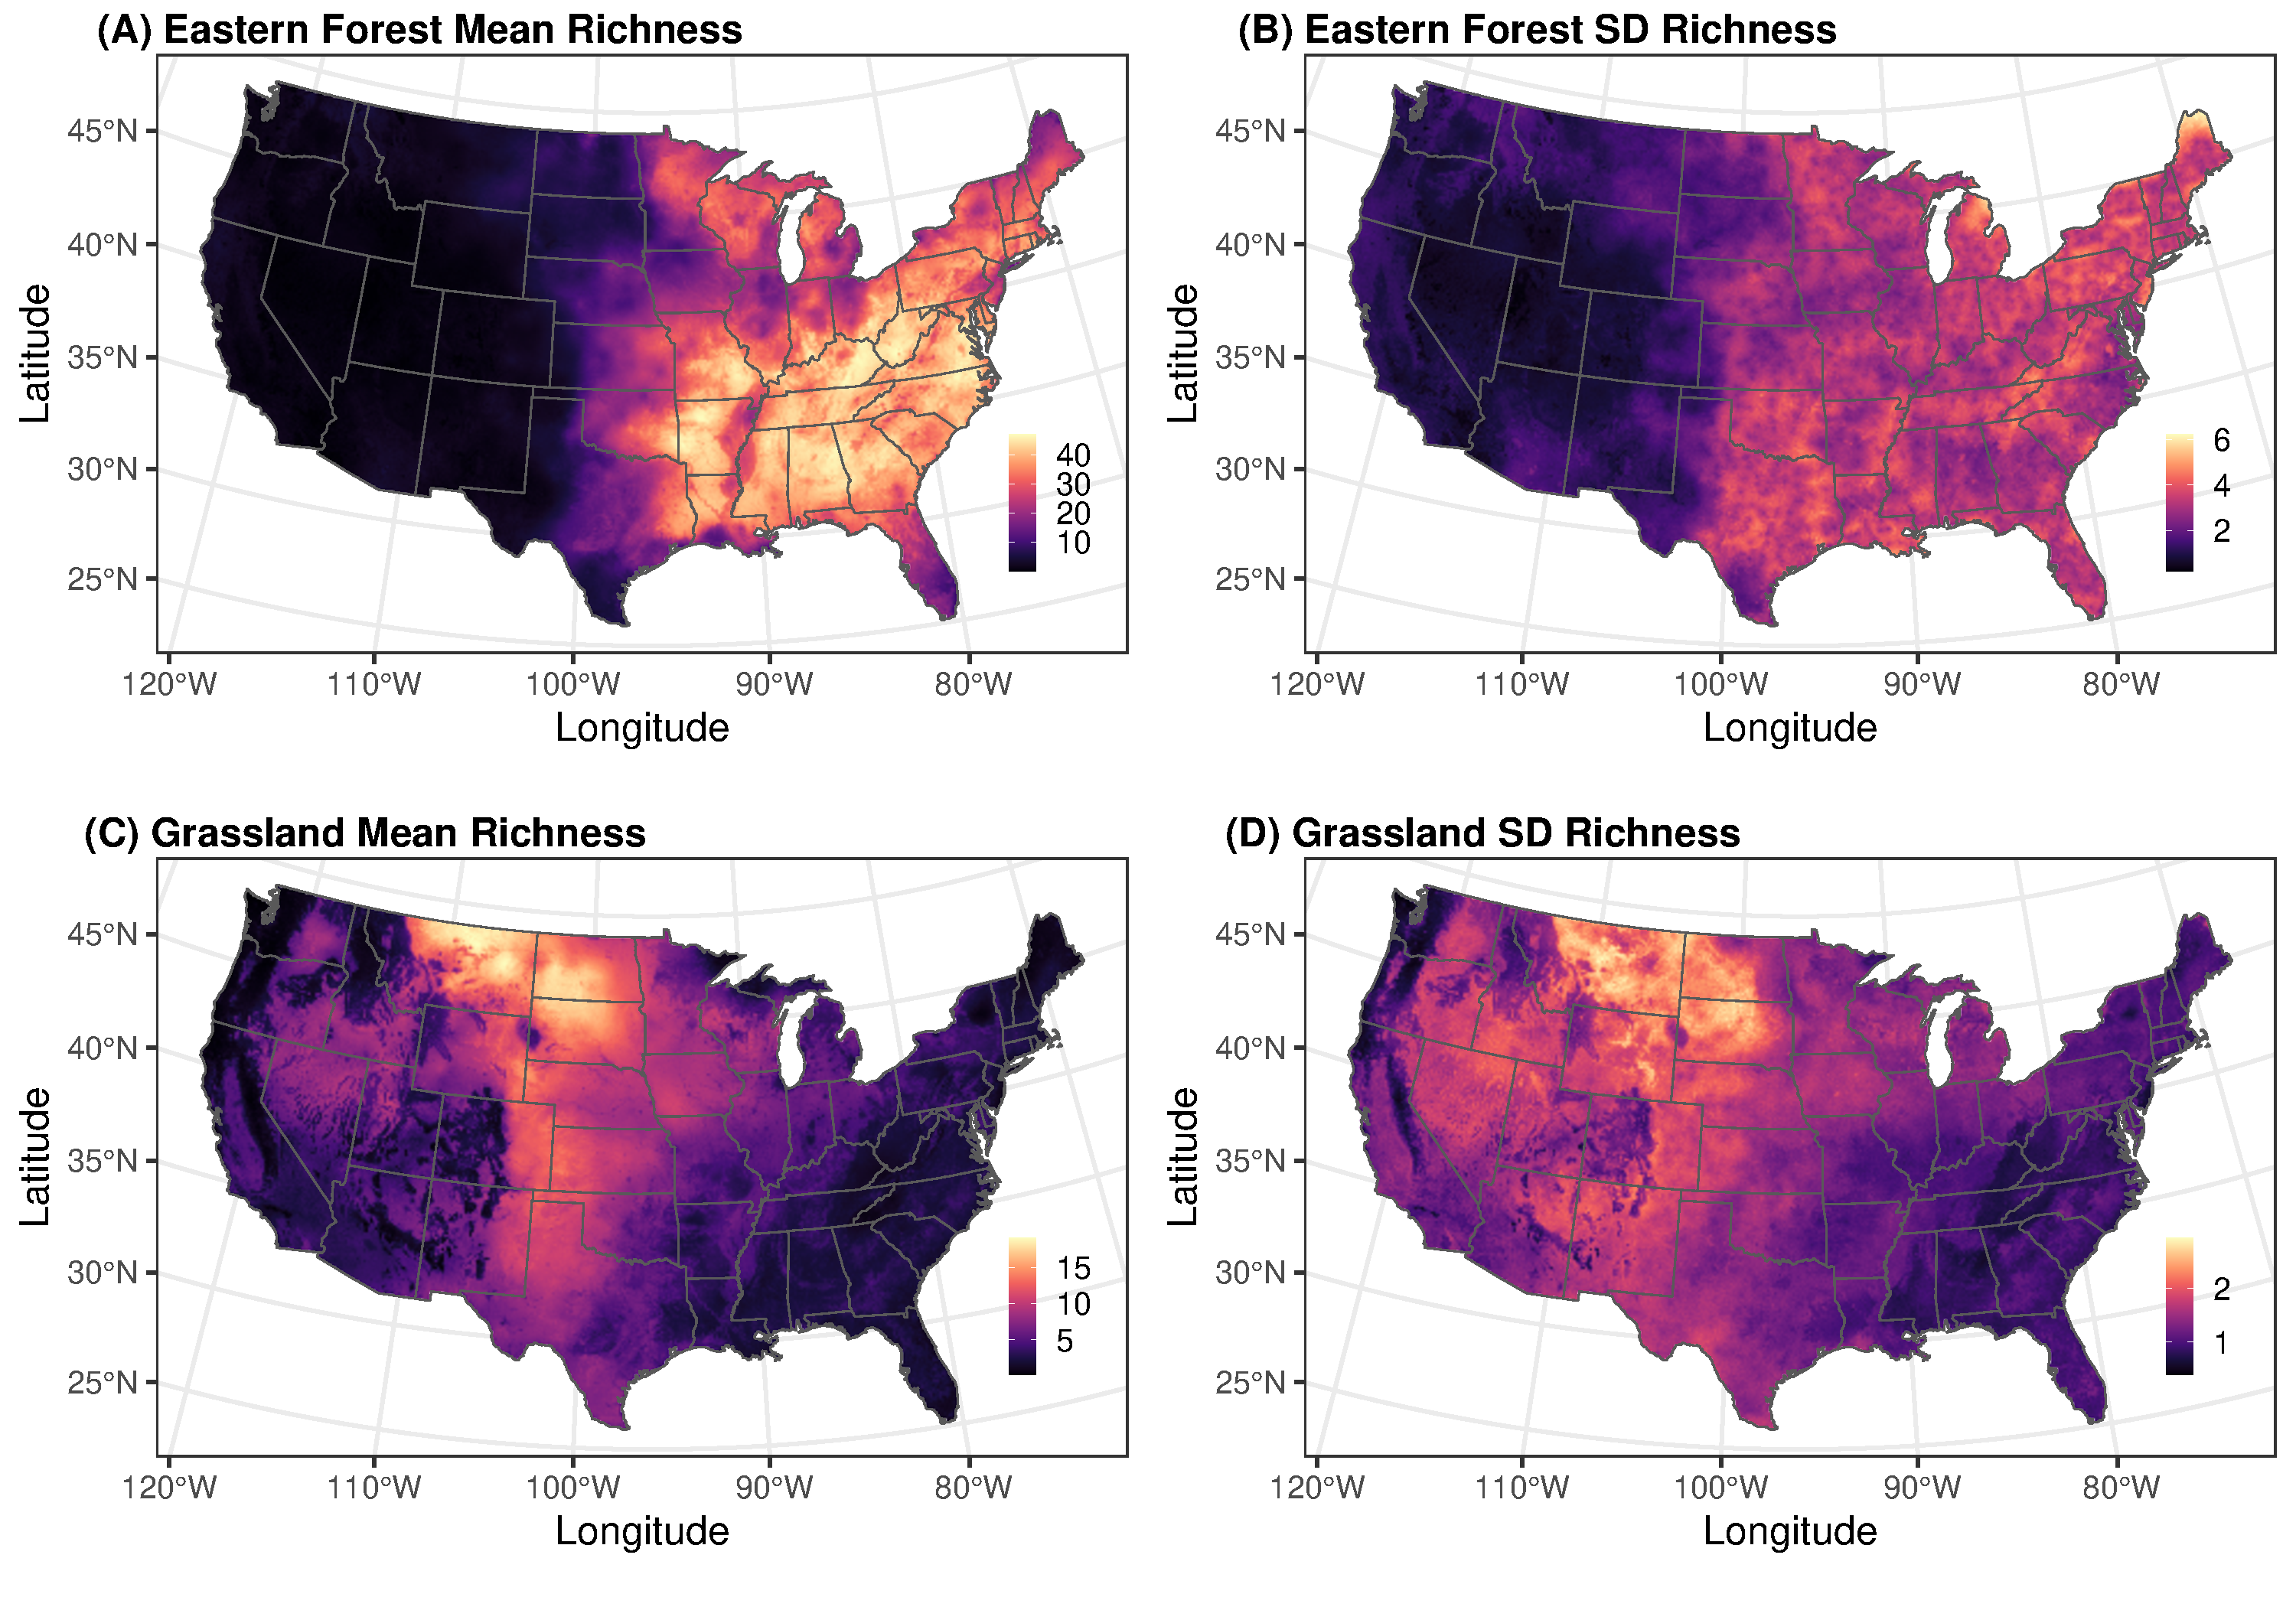
\includegraphics[width=11cm]{../figures/Fig1.pdf}
	\end{center}
\end{frame}

\begin{frame}{Example: bird communities across the continental US}
    Visualization of the first spatial factor and corresponding factor loadings
	\begin{center}
             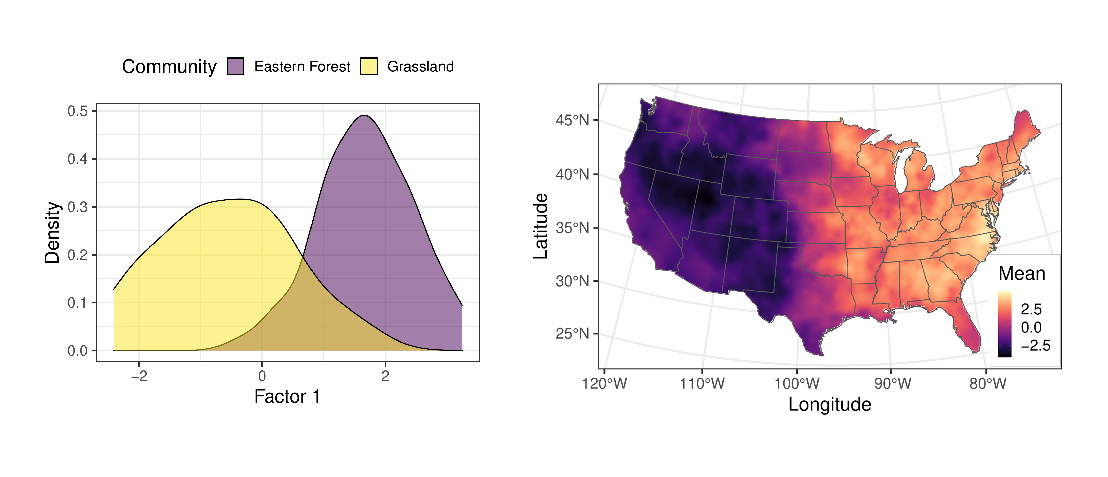
\includegraphics[width=11cm]{../figures/FigS1.pdf}
	\end{center}
\end{frame}

\begin{frame}{Some downsides to spatial factor models}
     \begin{itemize}
	     \item Convergence assessment is not always straightforward
	     \item Sensitivity to initial values 
	     \item Order of the first $q$ species has important implications for convergence and mixing.
	     \item Assume a multivariate stochastic process can be represented as a linear combination of independent univariate processes
     \end{itemize}
\end{frame}

\begin{frame}{Software}
   \begin{itemize}
        \item \texttt{spOccupancy}: spatial NNGP and non-spatial factor models for binary data
	\item \texttt{spAbundance}: Gaussian, Poisson, and NB spatial NNGP and non-spatial factor models.
	\item \texttt{boral}: many distributions for non-spatial and spatial factor models (Hui 2015 \textit{MEE}; spatial use full GPs fit in JAGS)
	\item \texttt{Hmsc}: spatial models using NNGPs (Tikhonov et al. 2019; \textit{MEE})
	\item \texttt{spBFA}: a variety of spatial models with some nifty priors (Berchuck et al. 2022 \textit{Bayesian Analysis})
   \end{itemize}
\end{frame}

\begin{frame}{Exercise}
	Modeling the distribution of 10 tree species across Vermont
\end{frame}

\end{document}
